%\documentclass[12pt,handout]{beamer}
\documentclass{beamer}
\usepackage[ngerman]{babel}
\usepackage[utf8]{inputenc}
\usepackage{amsmath}
\usepackage{amssymb}
\usepackage{listings} 
\usepackage{stmaryrd}
\lstset{language=Python, tabsize=4, showstringspaces=false,basicstyle=\tiny,mathescape=true}  
\lstset{literate=%
  {Ö}{{\"O}}1
  {Ä}{{\"A}}1
  {Ü}{{\"U}}1
  {ß}{{\ss}}1
  {ü}{{\"u}}1
  {ä}{{\"a}}1
  {ö}{{\"o}}1
}
\usepackage{mathtools}
\usepackage{ulem}
\usepackage{tikz}

\usetheme{Boadilla}
\mode<presentation>{
\useoutertheme[subsection=false]{miniframes}
\useinnertheme{rectangles}
%\usecolortheme{crane}
}
\parskip 10pt



\begin{document}
\title{Informatik}   
\author{Abstrakte Datentypen - Liste} 
\date{}
\frame{\titlepage} 

%---

\begin{frame}[fragile]

Abstrakter Datentyp (ADT) = Datenstruktur + (abstrakte) Operationen 

abstrakt = nicht implementiert, nur Vorgaben.  \pause

Beschreibung von Datenstrukturen unabhängig von ihrer späteren Implementierung in einer Programmiersprache.

ADTs bilden eine Spezifikation der Schnittstelle nach außen, indem sie Operationen und ihre Funktionalität festlegen
\end{frame}

%---

\begin{frame}[fragile]

ADT Liste

Definition: eine Liste ist eine (ggf. leere) Folge von Elementen zusammen mit einem so genannten 
(ggf. undefinierten) aktuellen Element. 

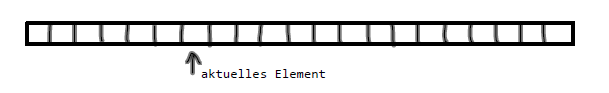
\includegraphics[scale=0.6]{bild1.png}  

Schnittstelle der ADT Liste:

\tiny
\begin{tabular}{l l l}
 empty & :  & liefert true, falls Liste leer  \\
 endpos & : & liefert true, wenn Liste abgearbeitet \\
 reset & :  &  das erste Listenelement wird zum aktuellen Element \\
 advance & : &  der Nachfolger des akt. wird akt. Element \\
 elem & : & liefert das aktuelle Element \\
 insert & : & fügt vor das aktuelle Element ein Element ein, das neue wird zum aktuellen Element \\
 delete & : & löscht das aktuelle Element, der Nachfolger wird zum aktuellen Element. \\
\end{tabular}


\end{frame}

%---

\begin{frame}[fragile]
\footnotesize 
\begin{lstlisting} 
class Liste:
    '''  Eine Liste ist eine (ggf. leere) Folge von Elementen zusammen mit einem
    (ggf. undefinierten) aktuellen Element  '''
    
    def empty(self):
        ''' liefert true, falls Liste leer '''
        pass
        
    def endpos(self):
        ''' liefert true, wenn die Liste abgearbeitet ist '''
        pass

    def reset(self):
        ''' das erste Listenelement wird aktuelles Element '''
        pass
    
    def advance(self):
        '''  der Nachfolger des aktuellen Elements wird aktuelles Element '''
        pass

    def elem(self):
        ''' liefert das aktuelle Element '''
        pass
  
    def insert(self, x):
        ''' Fügt x vor dem aktuellen Element ein, x wird zum neuen aktuellen Element. '''
        pass

    def delete(self):
        ''' löscht das aktuelle Element. Der Nachfolger wird neues aktuelles Element. '''
        pass

\end{lstlisting} 
\end{frame}

%---

\begin{frame}[fragile]


Implementation durch verkettete Einträge    

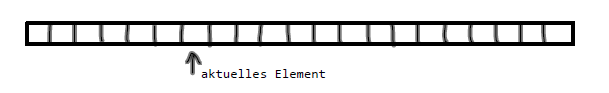
\includegraphics[scale=0.6]{bild1.png}  

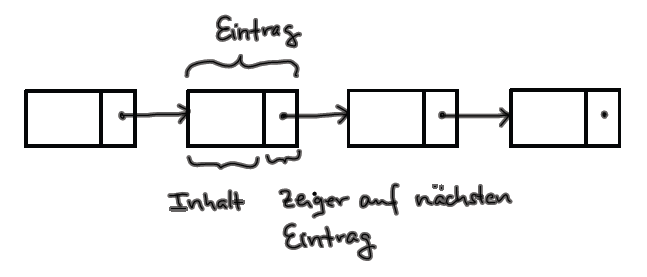
\includegraphics[scale=0.6]{bild2.png}  

\footnotesize 
\begin{lstlisting} 
class Eintrag: $\pause$
    def __init__(self):
        self.inhalt = None
        self.next = None
\end{lstlisting}

\end{frame}



\begin{frame}[fragile]
Problem bei der Implementation von insert:

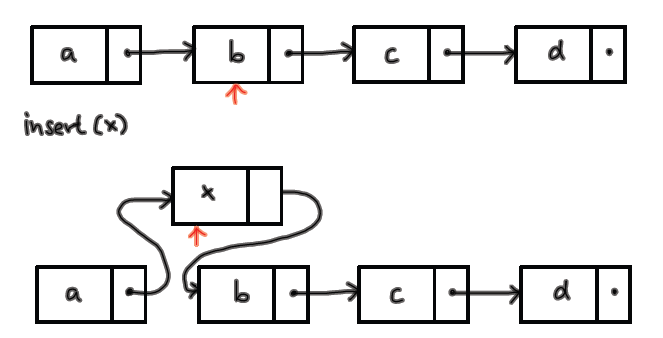
\includegraphics[scale=0.6]{bild4.png} \pause

Wie kann man den Zeiger, der auf das aktuelle Element zeigt, auf x umbiegen?
\end{frame}


%---
\begin{frame}[fragile]

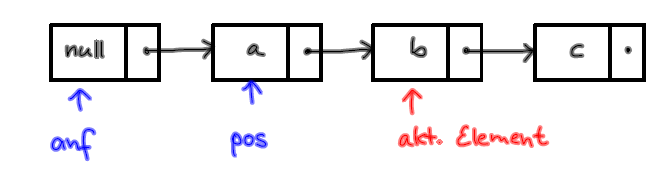
\includegraphics[scale=0.6]{bild5.png}  

\textit{pos} zeigt auf den Listen-Eintrag vor dem aktuellen Element.   

\textit{anf} zeigt auf einen dummy Eintrag vor dem ersten Element.

\end{frame}

\begin{frame}[fragile]
Mit assert-Anweisungen können wir unsere Implementation überprüfen
\footnotesize 
\begin{lstlisting} 
li = Liste()
assert li.empty()
assert li.endpos()
li.insert('A')
assert not li.empty()
assert not li.endpos()
assert li.elem() $==$ 'A'
li.advance()
assert li.endpos()
li.insert('B')
assert not li.endpos()
li.advance()
li.insert('C')
li.reset()
assert li.elem() $==$ 'A'
li.advance()
li.delete()
assert li.elem() $==$ 'C'
li.delete()
assert li.endpos()
li.reset()
li.delete()
assert li.empty()
\end{lstlisting} 
Bei einer nicht-leeren Liste können wir, wenn das aktuelle Element das letzte Element der Liste ist, mit
advance() noch einen Schritt vorangehen. Danach ist endpos() True, pos zeigt auf das letzte Element und
das aktuelle Element ist schon "jenseits der Liste".
 
\end{frame}


%---
\begin{frame}[fragile]
Nach der Implementation 
\footnotesize 
\begin{lstlisting} 
class Liste:
    def __init__(self):   $\pause$
        self.anf = Eintrag()
        self.pos = self.anf
       
    def empty(self):  $\pause$
        return self.anf.next is None
    
    def endpos(self): $\pause$
        return self.pos.next is None

    def reset(self): $\pause$
        self.pos = self.anf

    def advance(self): $\pause$
        if self.endpos(): raise RuntimeError("Fehler: Liste am Ende")
        self.pos = self.pos.next

    def elem(self): $\pause$
        if self.endpos(): raise RuntimeError("Fehler: Liste am Ende")
        return self.pos.next.inhalt

    def insert(self, x): $\pause$
        hilf = Eintrag()
        hilf.inhalt = x
        hilf.next = self.pos.next
        self.pos.next = hilf

    def delete(self): $\pause$
        if self.endpos(): raise RuntimeError("Fehler: Liste am Ende")
        self.pos.next = self.pos.next.next
\end{lstlisting} 
\end{frame}




 \end{document}